\documentclass{article}
% \usepackage{graphicx} % Required for inserting images
\usepackage[margin=20truemm]{geometry}
\usepackage[dvipdfmx]{graphicx}

\title{まとめ of An integrated model for aquaculture production, pathogen interaction, and environment effects}
\author{ウイルスマニア}
\begin{document}

\maketitle

\setlength{\baselineskip}{18pt}

\section*{初めに}
ABCフレームワークはA(Aquaculture: 養殖), B(Biosecurity: 環境守るやつ), C(Carrying Capacity: 環境収容力)の3つを含めた養殖における感染症の効果を含めた大規模な数理モデルフレームワークである。\\
あと脱線すると、数理モデルの論文を読むときはマテメソだけ読むと良い。\\
そんなことはまあどうでもいいが、とりあえずこのABCモデルでは以下の6つの数理モデルが絡んでいる。
\begin{enumerate}
    \item 養殖場における物理的なモデル
    \item 牡蠣とかの産物の成長を表すモデル
    \item 最小個体数の推定モデル
    \item 自然死率を推定するモデル(体重に応じて自然死が定義できるらしい)
    \item 感染症シミュレーションのモデル(病原体粒子の運動)
    \item SEIRモデル
\end{enumerate}
では、説明していく〜!!!

\section{養殖場における物理的なモデル}
まあ、まずは式ですね。(本文Fig.2を参照しながらでオネシャス)\\
\begin{equation}
    \frac{\partial C}{\partial t} = -u \frac{\partial C}{\partial x}+k_y\frac{\partial^2 C}{\partial y^2}+f(C)
\end{equation}
$C$:水に溶け込んでる粒子の濃度、つまりウイルスとかの濃度\\
$t$:時刻\\
$(x, y)$:$x$は養殖ボックスを並べている方向, $y$は養殖ボックスに垂直な方向\\
$u$:養殖ボックス方向への流体の速度\\
$k_y$:養殖ボックスに垂直な方向に粒子分散する係数\\
$f(C)$:非保存的プロセス($f:Population\mapsto C$みたいな感じ)\\
\begin{equation}
    \frac{2k_y\Delta t}{(\Delta y)^2}\leq 1
\end{equation}
$\Delta t$:刻み時間\\
$\Delta y$:ちょっとずらした$y$\\
まず、式(1)は$x$軸方向に連ねた養殖場におけるCの瞬間時間における変化を表したもので、$x$軸については「移流」、$y$軸については「拡散」でウイルス量などが変化する。また、$f(C)$というCの量に応じてCが定まる抽象的な関数も加算されることでファーム全体のウイルス濃度などを定めている。\\
また、式(2)はCFL条件という伝播速度を吟味する式で、それを1で抑えるために逆数を取ったという感じ。\\
つまり、$\frac{2k_y\Delta t}{(\Delta y)^2} \ll 1$なら伝播速度クッソ速いし、$\frac{2k_y\Delta t}{(\Delta y)^2} \sim 1$なら亀みたいな速度ってこと。\\
\textbf{シミュレーションでは差分法/有限要素法なりで方程式(1)を数値計算して、環境中にどのようにウイルス粒子が分布するか確認する。}

\section{牡蠣とかの産物の成長を表すモデル}
これは、論文が見れてなくてちょっとわからない。ジョアン先生に相談中。

\section{最小個体数の推定モデル}
これは、\\
(i)同化効率のランダムな変更について\\
(ii)体重依存の死について\\
をモデリングしたらしいけど、結果だけ使えばいいので一旦飛ばす。

\section{自然死率を推定するモデル(体重に応じて自然死が定義できるらしい)}
自然死はどうやら、体重に応じて変わるらしい。(本文Fig.4参照)\\
この図は要は死んだ時の体重がどのように分布しているか表しているものらしく、
まあ、ガウス分布に従うと。\\
そこで、体重依存の致死「係数」を作るという試みを行ったらしい。\\
それが、
\begin{equation}
    \frac{d\mu _w}{dW} = -\alpha \mu _w
\end{equation}
で、これを解くと
\begin{equation}
    \mu _w = \mu _0 e^{-\alpha W} + m_b
\end{equation}
が得られるわけだが。
要は式(3)は体重がめっちゃ増えると$\mu _w$はめっちゃ小さくなることを表していて(体感として、稚貝から成貝になると環境適応力が上がるから死ににくくなる感じ?)、\textbf{シミュレーションするときはエージェントベースモデル的な感じで個々の体重を元にそれぞれの致死係数を算出しているらしい。おそらく、SEIRに入れる時に使う。}

\section{感染症シミュレーションのモデル(病原体粒子の運動)}
これには三つのフェーズがあって\\
(i)Target site内にウイルス粒子が輸送される動態(Fig1:添付図参照)\\
(ii)宿主生体内での動態\\
(iii)宿主生体外での動態\\
が考えられるらしい。\\
(i)については以下の4つの数式が重要である。\\
\begin{equation}
    L_s = A_sI_sS_s
\end{equation}
\begin{equation}
    t = \frac{d}{u_r}
\end{equation}
\begin{equation}
    \frac{dP_w}{dt} = -(k_b+k_p)P_w
\end{equation}
\begin{equation}
    QP_w = QP_0e^{-(k_b+k_p)t}
\end{equation}
式(5)\\
$A_s$:Source siteにおける全個体数\\
$I_s$:Source siteにおける感染した個体数\\
$S_s$:Source siteにおける個人が排出したウイルスの割合\\
つまり、$L_s$はSouce siteにおいて保有しているウイルス量みたいなもの。\\
式(6)\\
$d$:Souce siteとFarm areaの距離\\
$u_r$:残留物の速度\\
つまり、$t$はSource siteからFarm areaにウイルス粒子が運搬されるまでの時間。\\
式(7), (8)\\
$P_w$:水中(Target area)のウイルス粒子の濃度\\
$P_0$:初期値\\
$k_b$:ウイルス自滅率的な感じのパラメータ\\
$k_p$:水中で分散することによるウイルス量の希釈パラメータ\\
$Q$:移流を特徴づけるよくわからない数字\\
このとき、式(5)を参照すると、$QP_w = L_t$(Target areaに到達したウイルス量=Target areaで積載しているウイルス量)と$QP_0 = L_s$(Source siteにいるウイルス量=Source siteで積載しているウイルス量)であることがわかる。

\section{SEIRモデル}
$f(C)$についても議論しなければ式(1)を語ることができない。\\
そこで、以下の式を考えている。
\begin{equation}
    Vf(C) = \tau B_e + \phi B_i - \sigma B_t
\end{equation}
$V$:ケージ体積\\
$\tau$:Exposedが排出するウイルス量(持続感染)\\
$B_e$:Exposedの個体数\\
$\phi$:Infectedが排出するウイルス量(溶解感染)\\
$B_i$:Infectedの個体数\\
$\sigma$:ウイルス量の増加率\\
$B_t$:Susceptible+Exposed+Infectedの全て。(Target areaの全個体数)\\
つまり、$f(C)$はウイルス濃度を表しており、$f:Population\mapsto C$を表している。\\
(個人的には、ここウイルス濃度を独立変数として取ってないから$f(C)$という表記はおかしい気がする。)\\

では最後に、SEIRモデルの一番重要な$\beta$についてを語る。\\
\begin{equation}
    \beta _p = \frac{P^\alpha _w}{ID50^\alpha + P^\alpha _w}
\end{equation}
$\beta _p$:感染の確率(感染係数ってやつ)\\
$\alpha$:Hillの式という反応速度論でよく使う式におけるシグモイド係数ってやつ(つまり、どれくらいグラフがS字に近いかってやつ)\\
$ID_{50}$:ウイルス学で使われるウイルス力価を推定する手法。具体的にはその場にある細胞やら個体やらの半数に感染させるのに必要なウイルス量。他には$TCID_{50}$なんかもある。
\begin{figure}[htbp]
    \centering
    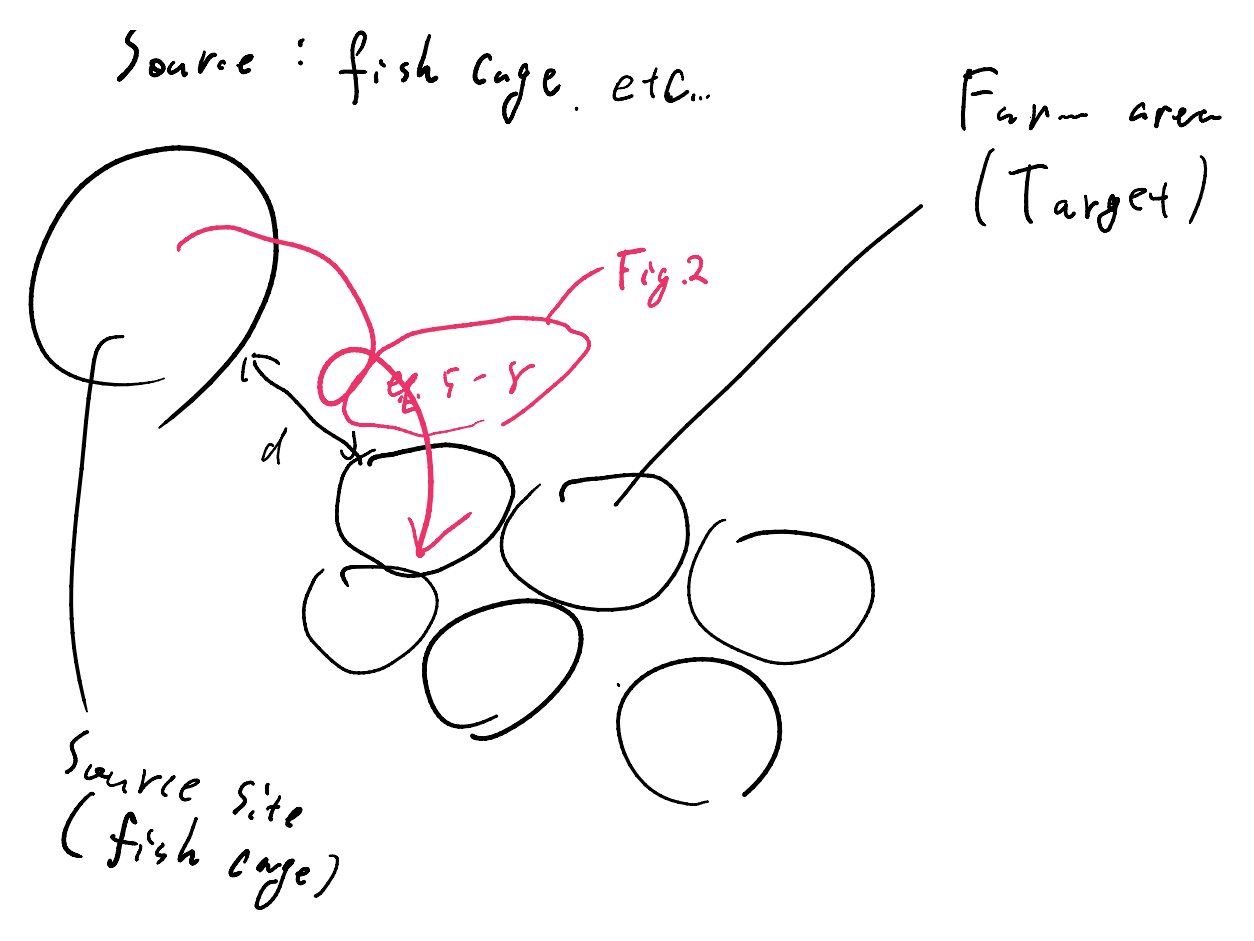
\includegraphics[width=\linewidth]{index_image1.png}
    \caption{添付図}
    \label{fig:enter-label}
\end{figure}
\end{document}
